\chapter{Diseño del sistema}
\section{Arquitectura}
La aplicación utiliza un proyecto MAUI de estilo SDK con interfaz XAML y código C\#. El punto de arranque se configura en \texttt{MauiProgram}; \texttt{App} crea la ventana, \texttt{AppShell} establece la página inicial y \texttt{MainPage} construye y coordina la interfaz del juego. \texttt{UnbeatableAIController} calcula la jugada sin manipular controles visuales.

Las cuatro figuras se generaron con Mermaid. Sus fuentes editables \texttt{01\_arquitectura.mmd}, \texttt{02\_casos\_de\_uso.mmd}, \texttt{03\_secuencia\_turno.mmd} y \texttt{04\_diagrama\_clases.mmd} se incluyen en el directorio \ruta{diagramas\_mermaid}.

\begin{figure}[!htbp]
\centering
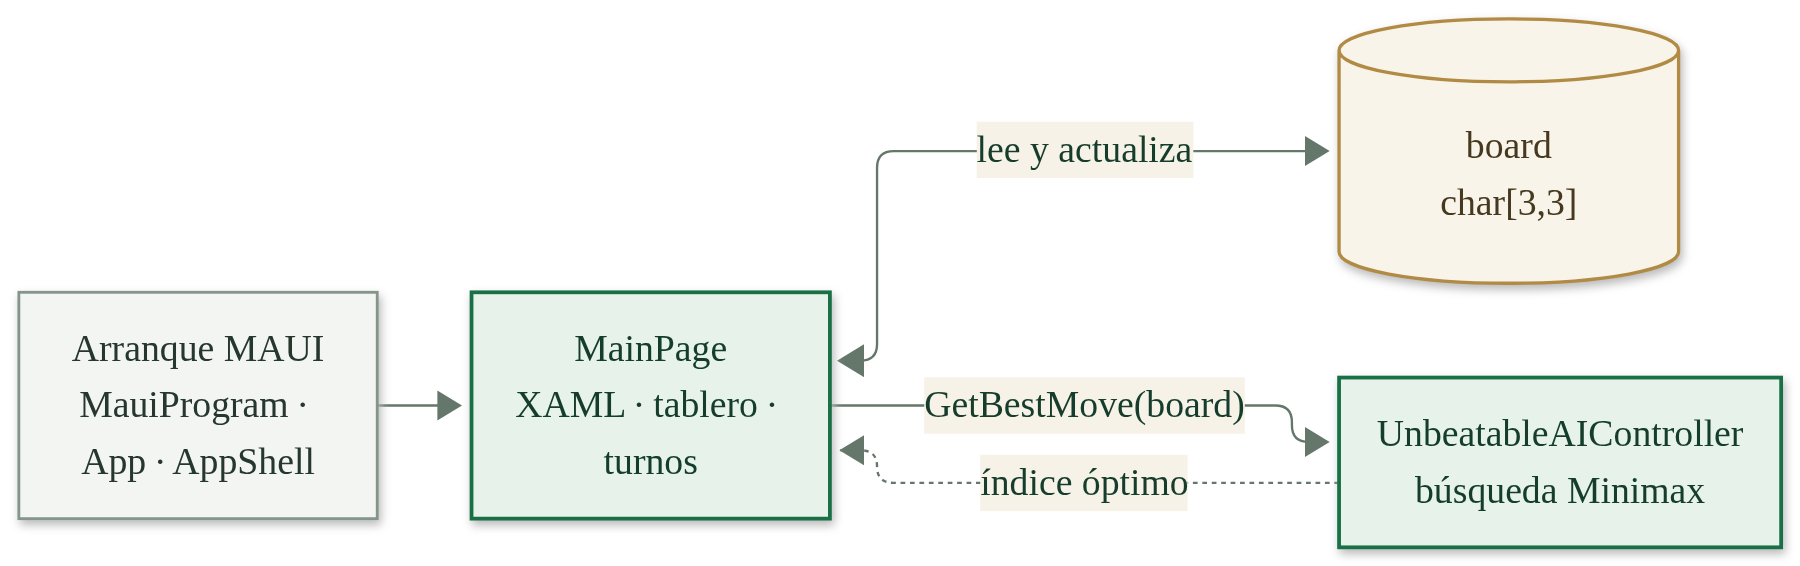
\includegraphics[width=0.92\textwidth,height=0.34\textheight,keepaspectratio]{figuras/diagramas_mermaid/01_arquitectura.png}
\caption[Arquitectura lógica de la aplicación MAUI]{Arquitectura lógica de la aplicación MAUI.}
\label{fig:arquitectura}
\end{figure}

\section{Representación del tablero}
La clase de página mantiene una matriz \texttt{char[3,3]} y un arreglo de nueve botones. Un índice lineal $i$ se convierte a coordenadas usando fila $i/3$ y columna $i\bmod 3$. En XAML la columna se calcula con $i\bmod 3$ y la fila con $i/3$. La matriz y la interfaz se actualizan en el mismo movimiento.

\begin{table}[H]
\centering
\caption{Relación entre índice lineal y coordenadas del tablero}
\label{tab:board-index}
\begin{tabular}{P{2.8cm}P{4.0cm}P{2.5cm}}
\toprule
\thd{Índices} & \thd{Fila de matriz} & \thd{Controles}\\
\midrule
0, 1, 2 & 0 & 1, 2, 3\\
3, 4, 5 & 1 & 4, 5, 6\\
6, 7, 8 & 2 & 7, 8, 9\\
\bottomrule
\end{tabular}
\end{table}

\section{Diagrama de casos de uso}
El actor es una persona que inicia una partida, marca casillas, reinicia, abre los menús o sale. La IA es un servicio interno invocado desde el flujo de una jugada; no es un segundo usuario externo.

\begin{figure}[!htbp]
\centering
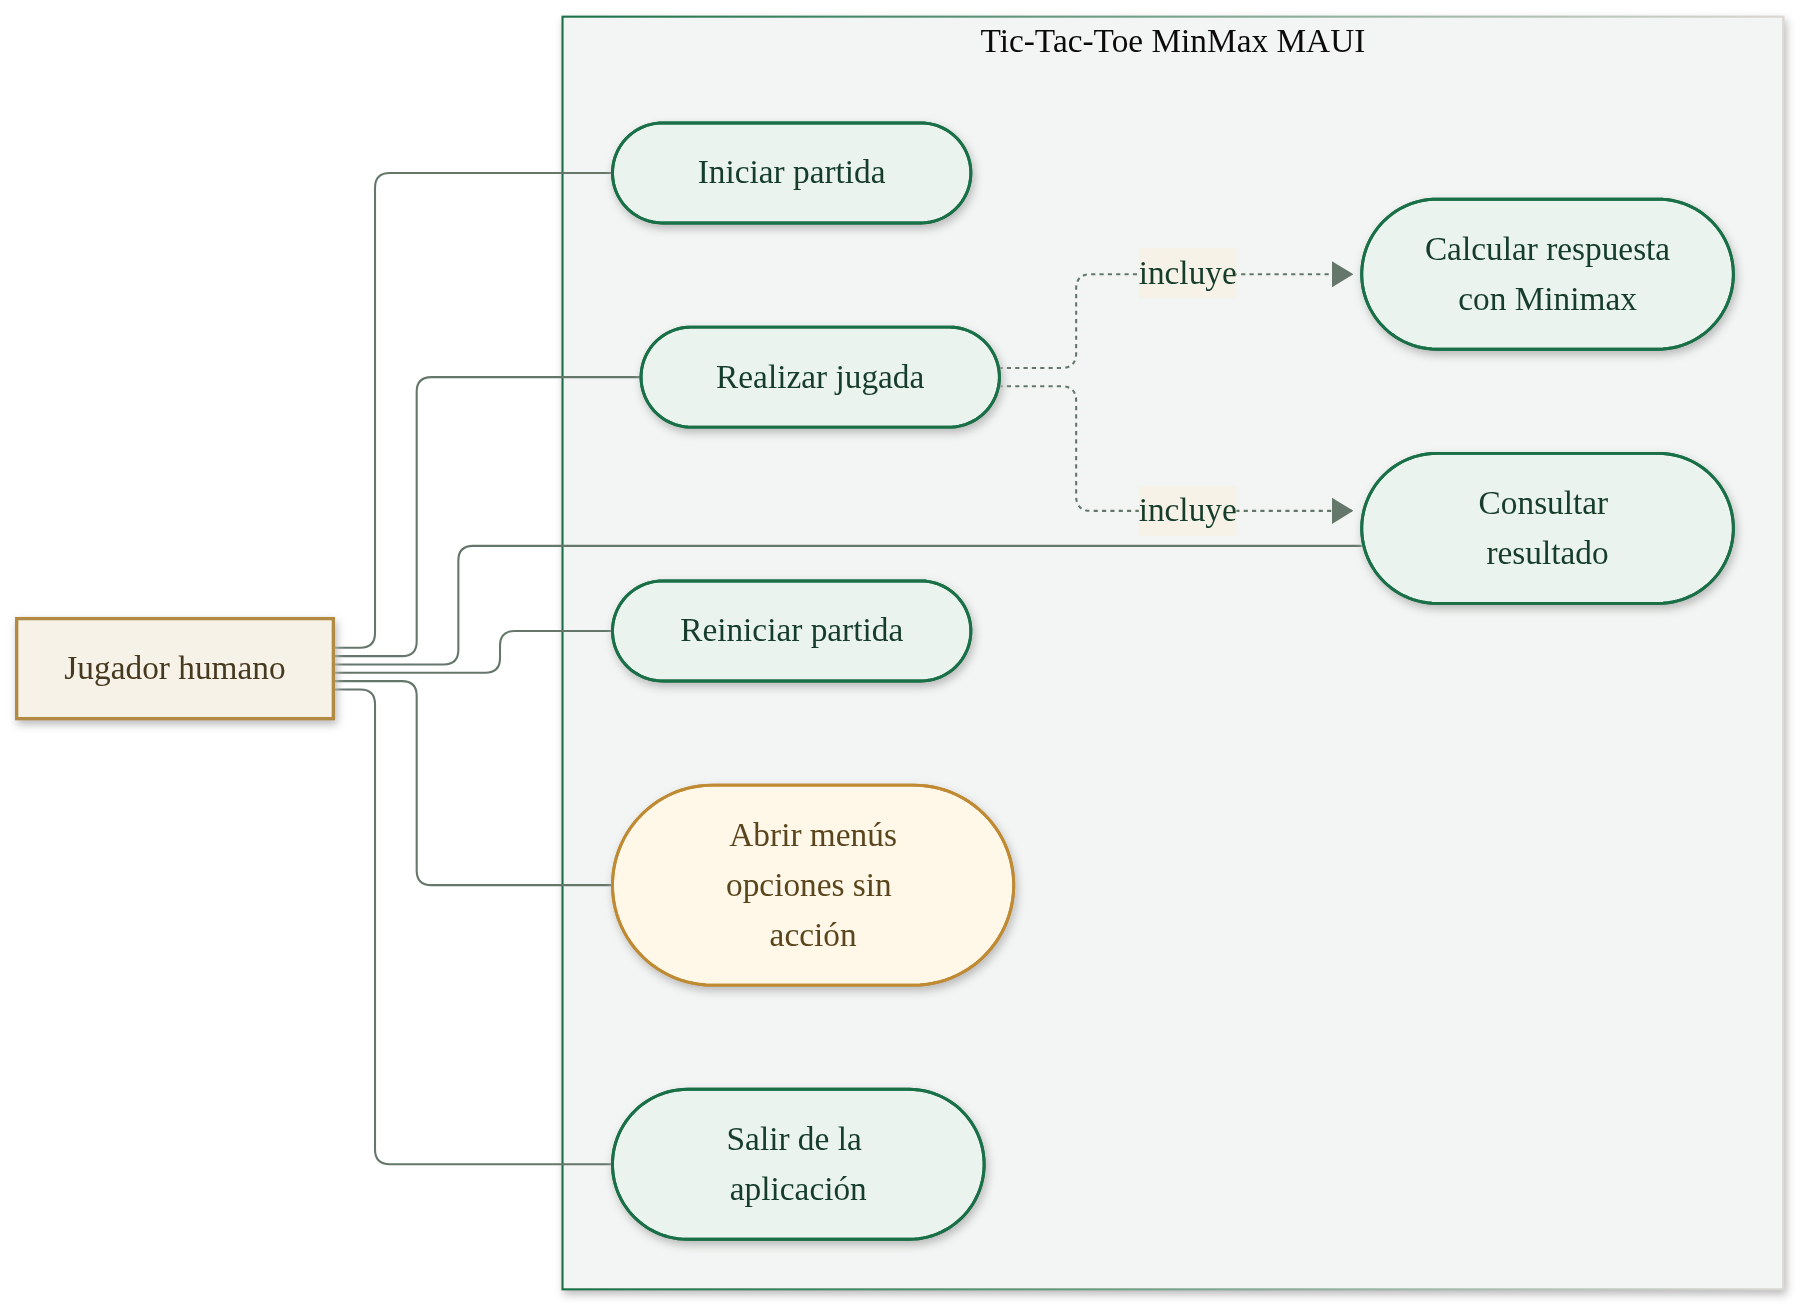
\includegraphics[width=0.96\textwidth,height=0.48\textheight,keepaspectratio]{figuras/diagramas_mermaid/02_casos_de_uso.png}
\caption[Casos de uso de la aplicación]{Casos de uso visibles. La selección de opciones internas de menú está pendiente.}
\label{fig:usecases}
\end{figure}

\subsection{Descripción resumida de casos de uso}
\begin{table}[H]
\centering
\small
\caption{Casos de uso y condición observada}\label{tab:usecases}
\begin{tabular}{P{1.3cm}P{3.1cm}P{8.9cm}}
\toprule
\thd{ID} & \thd{Caso} & \thd{Flujo principal}\\
\midrule
CU-01 & Iniciar partida & La página inicializa el tablero vacío, habilita las casillas y entrega el primer turno a \texttt{X}.\\
CU-02 & Realizar jugada & La persona toca una casilla disponible; el programa escribe \texttt{X}, revisa el fin de partida y solicita la jugada de \texttt{O}.\\
CU-03 & Consultar resultado & Tras cada jugada se buscan líneas ganadoras y se comprueba si el tablero está lleno; si corresponde, se muestra un aviso.\\
CU-04 & Reiniciar & El botón Nuevo borra la matriz y los textos de los botones, los habilita y devuelve el turno a la persona.\\
CU-05 & Abrir menú & Archivo, Ver o Ayuda muestran una hoja de acciones. Elegir una opción no ejecuta una acción en el código actual.\\
CU-06 & Salir & El botón Salir invoca el cierre de la aplicación.\\
\bottomrule
\end{tabular}
\end{table}

\section{Diagrama de secuencia de una jugada}
\begin{figure}[!htbp]
\centering
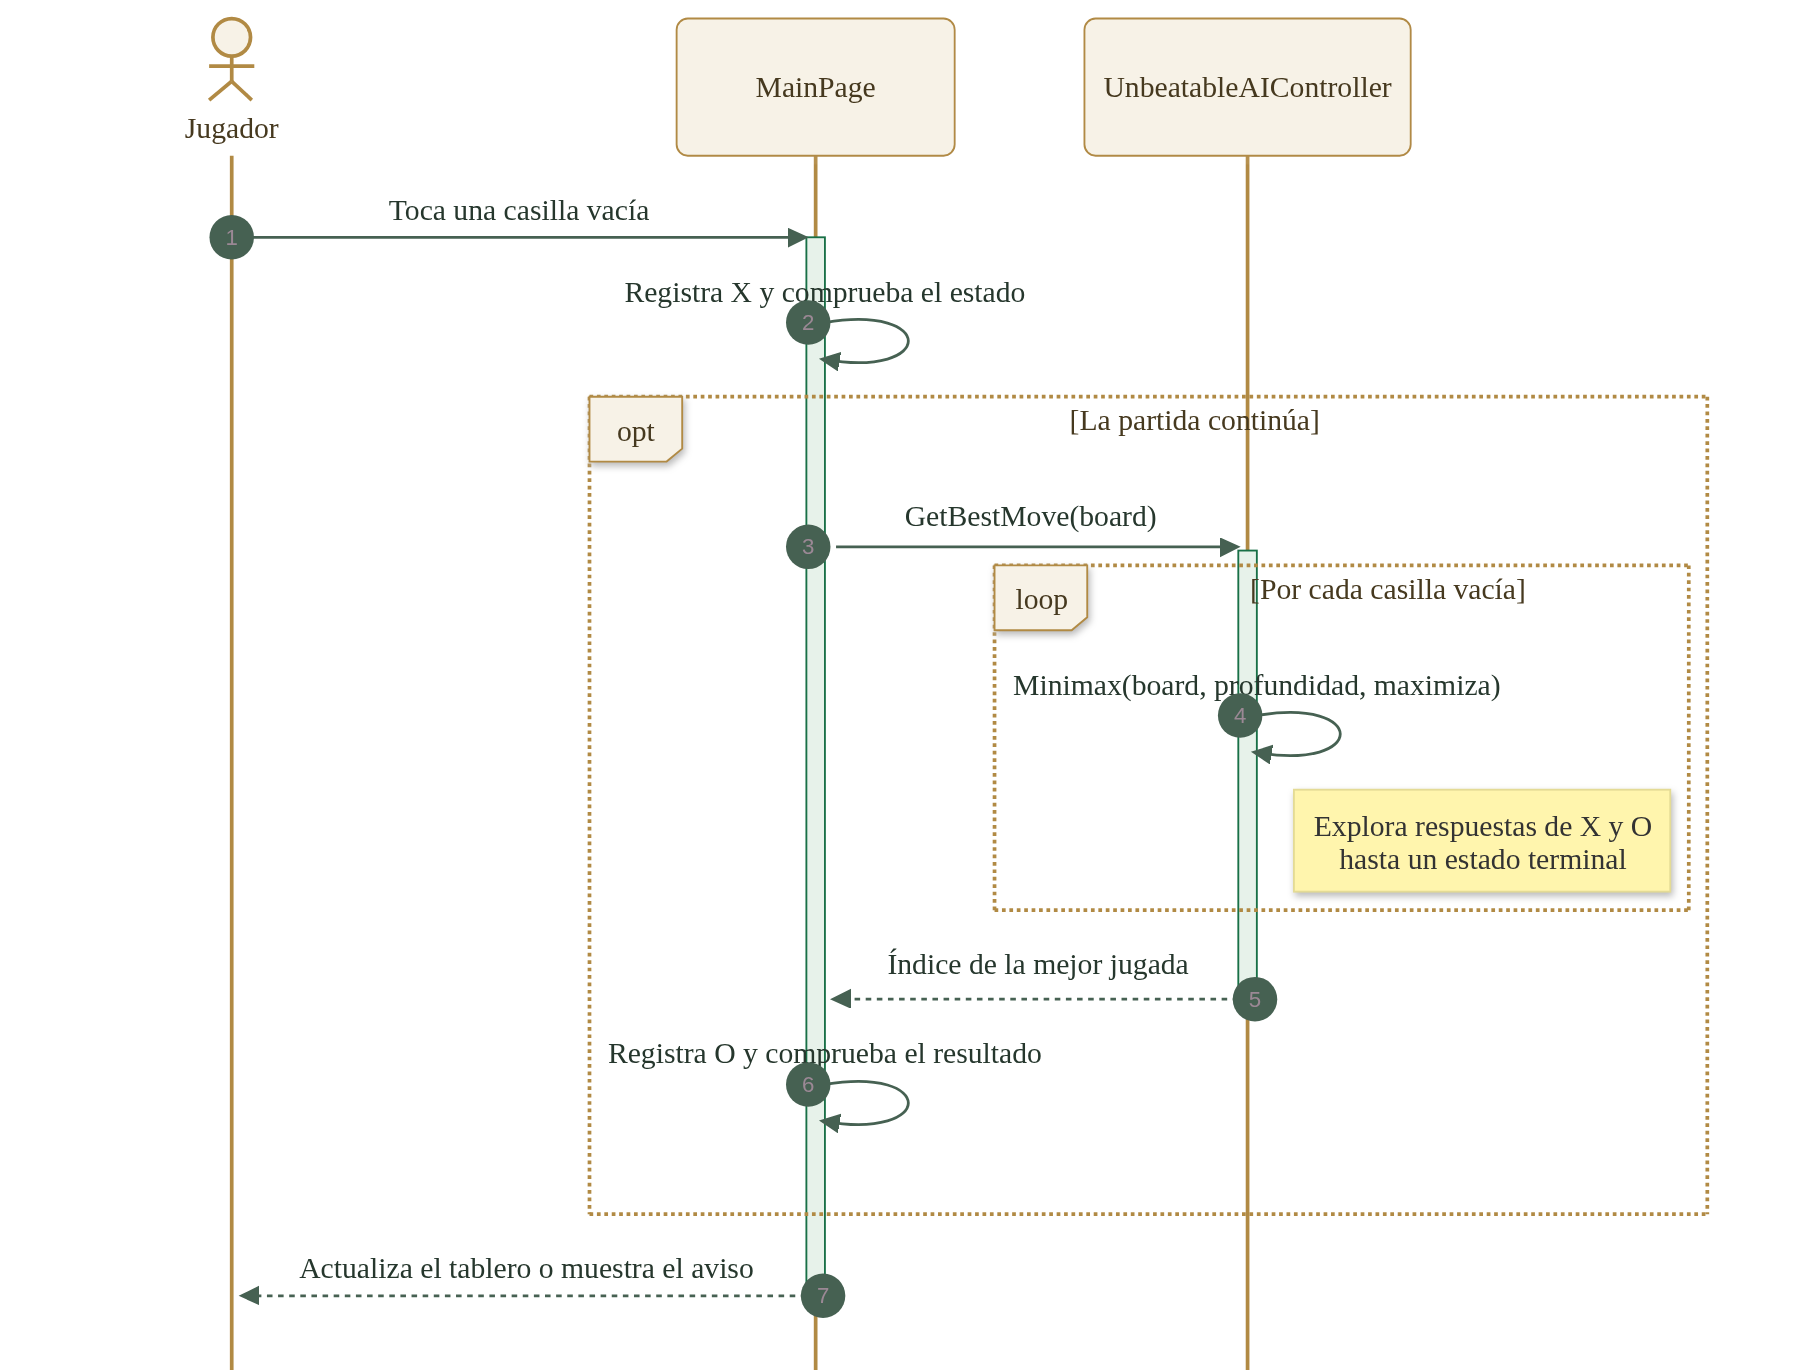
\includegraphics[width=0.92\textwidth,height=0.52\textheight,keepaspectratio]{figuras/diagramas_mermaid/03_secuencia_turno.png}
\caption[Secuencia de una jugada y búsqueda Minimax]{Secuencia de una jugada y búsqueda recursiva de la IA.}
\label{fig:sequence}
\end{figure}

\section{Diagrama de clases}
\begin{figure}[!htbp]
\centering
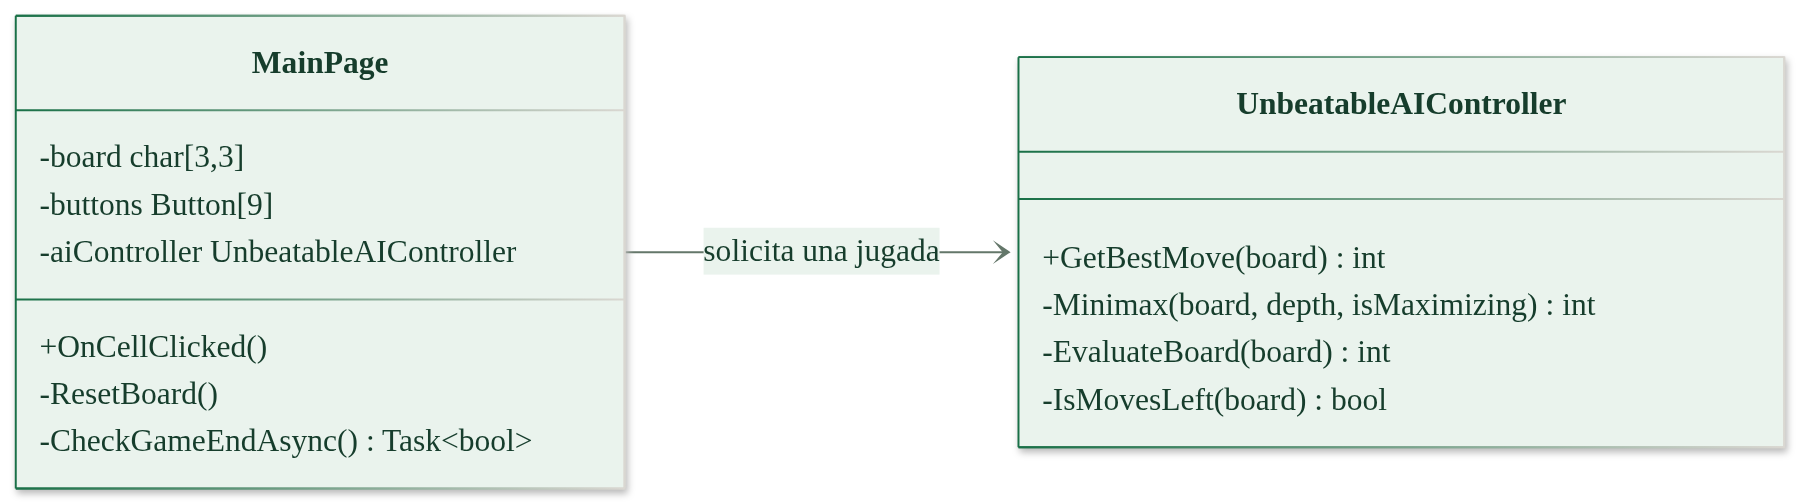
\includegraphics[width=0.98\textwidth,height=0.32\textheight,keepaspectratio]{figuras/diagramas_mermaid/04_diagrama_clases.png}
\caption[Clases centrales de la lógica del juego]{Clases centrales de la lógica del juego y dependencia de Minimax.}
\label{fig:classes}
\end{figure}

% ----------------------------------------------------------------------
